\documentclass[compress, 8pt]{beamer}
% \documentclass[handout, 8pt]{beamer}
\usepackage[utf8]{inputenc}

% Notes to self: \nts[color option]{text that is a note}
\newif\ifshowcomments
% \showcommentstrue % uncomment to show
\input{preambleB}
\usepackage[normalem]{ulem}

%%%%%%%%%%%%%%%%%%%%%%%%%%%%%%%%%%%%%%%%%%%%%%%%%%%%%%%%%%%%%%%%%%%%%%%%%%%%%%
% Paths to figures
\usepackage{subcaption}

% block quotes
\usepackage{csquotes}

% Avoid a warning on mac; can introduce a warning (and maybe a break) on windows
% \usepackage{etex}
% Avoid a warning
\let\Tiny=\tiny

%Information to be included in the title page:
\title{Synthetic Control}
\subtitle{ECON726}
\author[]{Tara Sullivan}
\institute{
Tara Sullivan \\
\textit{tara.sullivan55@login.cuny.edu}
}
\date{
\today
\nts{\\
\medskip
Notes/comments are in gray and will be excluded from the presentation.
}
}

% plot graphs with pgfplots
\usepackage{pgfplots}
\pgfplotsset{compat=newest}
\usepgfplotslibrary{groupplots}
\usepgfplotslibrary{dateplot}
\pgfplotsset{compat=newest,
    every axis/.style={
        axis y line*=left,
        axis x line*=bottom,
        % allows for multi-line legend entries
        legend style={cells={align=left}},
        % allows for multi-line titles
        title style={align=center},
    },
}

% For animations using underbrace 
% Source: https://tex.stackexchange.com/a/565866
\usepackage{xparse, letltxmacro}
\LetLtxMacro{\oldunderbrace}{\underbrace}
\DeclareDocumentCommand{\underbrace}{d<> m e{_}}{%
  \IfValueTF{#1}{% IF <overlay-specification> given
    % using global onlside flag, cf. p82 beamer manual v3.59
    \oldunderbrace{#2\onslide<#1>}_{#3}\onslide%
  }{% ELSE
    \oldunderbrace{#2}_{#3}
  }%
}%

\usetikzlibrary{decorations.pathreplacing,calligraphy}

%%%%%%%%%%%%%%%%%%%%%%%%%%%%%%%%%%%%%%%%%%%%%%%%%%%%%%%%%%%%%%%%%%%%%%%%%%%%%%%%
\begin{document}    
%\beamertemplatenavigationsymbolsempty


%%%%%%%%%%%%%%%%%%%%%%%%%%%%%%%%%%%%%%%%%%%%%%%%%%%%%%%%%%%%%%%%%%%%%%%%%%%%%%%%
\begin{frame}
\titlepage
% \tikzset{external/figure name={intro_}}
\end{frame}

%%%%%%%%%%%%%%%%%%%%%%%%%%%%%%%%%%%%%%%%%%%%%%%%%%%%%%%%%%%%%%%%%%%%%%%%%%%%%%%%
\begin{frame}{Housekeeping}

Homework:
\begin{itemize}
    \item Regression discontinuity designs next week (MHE Chp 6)
    \item Replication assignment due! Remember: we want primary results!
\end{itemize}

\end{frame}

%%%%%%%%%%%%%%%%%%%%%%%%%%%%%%%%%%%%%%%%%%%%%%%%%%%%%%%%%%%%%%%%%%%%%%%%%%%%%%%%
\begin{frame}{Empirical project}

\textbf{Paper selection}: Due \textbf{September 22} [5\% of final grade]
\begin{itemize}
\item Done! 
\end{itemize}

\textbf{Project plan}: Due \textbf{October 14} [15\% of final grade] 
\begin{itemize}
\item Done!
\end{itemize} 

\textbf{Replication results}: \textbf{November 3}: [10\% of final grade]
\begin{itemize}
\item You should submit some of your main replication results. The final results should be formatted as tables and charts in a word document or PDF, submitted on Brightspace. Your code and data should accessible on GitHub.
\end{itemize}

\textbf{Presentation}: Due \textbf{December 2} \& \textbf{December 9} [10\% of final grade]
\begin{itemize}
\item Prepare a 5-8 minute presentation on your paper. Focus on the research question, main result, and one extension. 
\end{itemize}

\textbf{Final Paper}: Due \textbf{December 16} [35\% of final grade]
\begin{itemize}
\item Your paper should contain 6-10 pages of text, and 3-6 pages of figures (double spaced, 12 point font).
You must provide the code and data to replicate your findings. 
Your final project should be submitted on Brightspace, and your code and data should be uploaded to github (note: if your data is too large to upload to github, let me know). 
\end{itemize}

\end{frame}



%%%%%%%%%%%%%%%%%%%%%%%%%%%%%%%%%%%%%%%%%%%%%%%%%%%%%%%%%%%%%%%%%%%%%%%%%%%%%%%
\miniframesoff
\begin{frame}{Outline}
    \tableofcontents
\end{frame}
\miniframeson



%%%%%%%%%%%%%%%%%%%%%%%%%%%%%%%%%%%%%%%%%%%%%%%%%%%%%%%%%%%%%%%%%%%%%%%%%%%%%%%%
\section[Diff-in-diff]{Differences-in-differences review}
\miniframesoff
\begin{frame}
    \tableofcontents[currentsection]
\end{frame}
\miniframeson
%%%%%%%%%%%%%%%%%%%%%%%%%%%%%%%%%%%%%%%%%%%%%%%%%%%%%%%%%%%%%%%%%%%%%%%%%%%%%%%%

%%%%%%%%%%%%%%%%%%%%%%%%%%%%%%%%%%%%%%%%%%%%%%%%%%%%%%%%%%%%%%%%%%%%%%%%%%%%%%%%
\begin{frame}{Diff-in-diff review (Card and Kruegr, 1994)}

Note: these notes are from my PhD course on Causal Inference, taught by \href{https://sites.google.com/site/wuethricheconomics/home?authuser=0}{Kaspar W{\"u}thrich}

\vspace{2ex}
Set-up:
\begin{itemize}
    \item Two groups (treatment and control): $G=1$ and $G=0$
    \item Two periods (before and after the treatment): $T=0$ and $T=1$
    \item Only one group is treated in one period
\end{itemize}
Data:
\begin{itemize}
    \item Survey of 400 fast food stores both in NJ and PA both before and after the minimum wage increase in NJ
\end{itemize}
Results:
\begin{itemize}
    \item Positive effect of increasing the minimum wage on employment
\end{itemize}

\end{frame}

%%%%%%%%%%%%%%%%%%%%%%%%%%%%%%%%%%%%%%%%%%%%%%%%%%%%%%%%%%%%%%%%%%%%%%%%%%%%%%%%
\begin{frame}{Formal analysis of simple DiD model}

Potential outcomes framework:
\begin{itemize}
    \item $D$: treatment indicator; $D = T \cdot G$
    \item $Y (d)$: potential outcome
    \item $Y$: observed outcome; $Y = D \cdot Y(1) + (1 - D) \cdot Y(0)$: 
\end{itemize}

\vspace{3ex}
\textbf{Key assumption: }

\emph{Common trends: $\EE [Y (0) \vert G, T = 1] - \EE [Y(0) \vert G, T=0]$ does not depend on $G$}

\vspace{3ex}
Under common trends assumption, average treatment effect on the treated defined as:
\begin{align*}
\Delta_{DiD} =& \EE [Y (1) - Y(0) \vert G=1, T=1] \\
=& \left(\EE [Y \vert G = 1, T = 1] - \EE [Y \vert G = 1, T= 0]\right) \\
&- \left( \EE [Y \vert G = 0, T = 1] - \EE [Y \vert G =0, T = 0] \right)
\end{align*}

Estimation can proceed based on the simple regression model:
\begin{equation*}
    Y = \alpha + \gamma G + \lambda T + \Delta_{DiD} D + \epsilon
\end{equation*}

\end{frame}

%%%%%%%%%%%%%%%%%%%%%%%%%%%%%%%%%%%%%%%%%%%%%%%%%%%%%%%%%%%%%%%%%%%%%%%%%%%%%%%%
\begin{frame}{Discussion and notes about diff-in-diff model}

\begin{itemize}
\item Common trends assumption requires that average outcomes for treated and controls would have followed \emph{parallel trends} in the absence of treatment

\vspace{4ex}
\item Assumption of common trends is fundamentally untestable. We can get some idea of its plausibility when several periods are available, by checking the pre-trends are the same for treated and controls

\vspace{4ex}
\item One can also run placebo tests, and include leads into a regression-based DiD model, to check the plausibility of the parallel trends assumption

\end{itemize}

\vspace{2ex} Let's move on to issues and challenges with diff-in-diff

\end{frame}

%%%%%%%%%%%%%%%%%%%%%%%%%%%%%%%%%%%%%%%%%%%%%%%%%%%%%%%%%%%%%%%%%%%%%%%%%%%%%%%%
\begin{frame}{Issue \#1: common trends and scaling}

The parallel trends assumption is \textbf{scale dependent}
\begin{itemize}
    \item Parallel trends won't hold both for $Y$ and a monotone function of $Y$ (like $\log (y)$) at the same time
\end{itemize}

\vspace{3ex}
How to overcome this issue:
\begin{itemize}
    \item Answer: Changes-in-changes model; see Athey and Imbens (2006)
\end{itemize}
\url{https://onlinelibrary.wiley.com/doi/abs/10.1111/j.1468-0262.2006.00668.x}

\vspace{3ex}
\begin{displayquote}
We... propose an estimator that can be applied using either repeated cross section or panel data. Our approach provides an estimate of the entire counterfactual distribution of outcomes that would have been experienced by the treatment group in the absence of the treatment and likewise for the untreated group in the presence of the treatment.
\end{displayquote}

\end{frame}

%%%%%%%%%%%%%%%%%%%%%%%%%%%%%%%%%%%%%%%%%%%%%%%%%%%%%%%%%%%%%%%%%%%%%%%%%%%%%%%%
\begin{frame}{Issue \#2: fuzzy designs}

Simple diff-in-diff assumes $D = T \cdot G$. Often, $D \neq T \cdot G$. Example: Duflo (2001)
\begin{itemize}
    \item Looking at primary school construction in Indonesia, to measure the returns to education
    \item Many primary schools were constructed in districts with few schools ($G=1$), and few new schools were constructed in districts with a lot of schools ($G=1$)
    \item Primary school completion rate increases more in $G=1$ than in $G=0$, but not from 0\% to 100\%
\end{itemize}

\vspace{3ex}
How to overcome this issue:
\begin{itemize}
    \item Answer: fuzzy differences-in-differences; see de Chaisemartin and D'Haultfoeuille (2018)
\end{itemize}
\url{https://academic.oup.com/restud/article-abstract/85/2/999/4096388}
\end{frame}

%%%%%%%%%%%%%%%%%%%%%%%%%%%%%%%%%%%%%%%%%%%%%%%%%%%%%%%%%%%%%%%%%%%%%%%%%%%%%%%%
\begin{frame}{Issue \#3: choice of control group}

Simple diff-in-diff model assumes a control group with common trends exists

\vspace{3ex}
How do we choose a control group if there are multiple options?
\begin{itemize}
    \item Synthetic control!
\end{itemize}

\end{frame}



%%%%%%%%%%%%%%%%%%%%%%%%%%%%%%%%%%%%%%%%%%%%%%%%%%%%%%%%%%%%%%%%%%%%%%%%%%%%%%%%
\section[Synthetic Control]{Synthetic Control}
\miniframesoff
\begin{frame}
    \tableofcontents[currentsection]
\end{frame}
\miniframeson
%%%%%%%%%%%%%%%%%%%%%%%%%%%%%%%%%%%%%%%%%%%%%%%%%%%%%%%%%%%%%%%%%%%%%%%%%%%%%%%%


%%%%%%%%%%%%%%%%%%%%%%%%%%%%%%%%%%%%%%%%%%%%%%%%%%%%%%%%%%%%%%%%%%%%%%%%%%%%%%%%
\begin{frame}{Synthetic Control}

\href{https://pubs.aeaweb.org/doi/pdfplus/10.1257/jep.31.2.3}{Athey and Imbens (2017)}
\begin{displayquote}[pg. 3]
Synthetic control is ``arguably the most important innovation in the policy evaluation literature in the last 15 years.''
\end{displayquote}

\vspace{2ex}
First developed in \href{https://www.aeaweb.org/articles?id=10.1257/000282803321455188}{Abadie and Gardeazabal (2003)}
\begin{itemize}
    \item Study effect of terrorism on aggregate income
\end{itemize}

\vspace{2ex}
Formalized in \href{https://www.jstor.org/stable/29747059?seq=1}{Abadie, Diamond, and Hainmueller (2010)}
\begin{itemize}
    \item Impact of Prop 99 on smoking in California
\end{itemize}

\vspace{2ex}
Formalized in the comparative politics literature in \href{https://onlinelibrary.wiley.com/doi/abs/10.1111/ajps.12116}{Abadie, Diamond, and Hainmueller (2014)}
\begin{itemize}
    \item Impact of German reunification on West Germany
\end{itemize}


\end{frame}


%%%%%%%%%%%%%%%%%%%%%%%%%%%%%%%%%%%%%%%%%%%%%%%%%%%%%%%%%%%%%%%%%%%%%%%%%%%%%%%%
\begin{frame}{Example motivating synthetic control: Mariel boatlift}

\href{https://www.jstor.org/stable/2523702}{Card (1990)}: Do inflows of immigrants depress wages and the employment of natives in local labor markets?


\vspace{2ex} 
Context: Mass immigration of Cubans from Cuba's Mariel Harbor to the US between April and October 1980
\begin{itemize}
    \item In 1980, Fidel Castro announced anyone wishing to leave Cuba could do so

    \item 125,000 Cubans emigrated to Florida over six months

    \item Increased the Miami labor force by 7\%
\end{itemize}

\vspace{2ex}
Viewed as a natural experiment; Mariel boatlift provided an exogenous shift in labor supply
\begin{itemize}
    \item Used individual-level data CPS data on unemployment from four comparison cities (Atlanta, LA, Houston, Tampa)
    \item Claims cities are comparable based on demographics and economic conditions
    \item Estimated diff-in-diff model
\end{itemize}

\vspace{2ex}
Outcome: results were contrary to competitive labor-market model
\begin{displayquote}[]
The Mariel influx appears to have had virtually no effect on the wages or unemployment rates of less-skilled workers, even among Cubans who had immigrated earlier
\end{displayquote}

\end{frame}

%%%%%%%%%%%%%%%%%%%%%%%%%%%%%%%%%%%%%%%%%%%%%%%%%%%%%%%%%%%%%%%%%%%%%%%%%%%%%%%%
\begin{frame}{Critique of Card (1990)}

Empirical critiques of Card (1990):
\begin{itemize}
    \item Choice of control was subjective
    \item Standard errors reflect sampling variance, as opposed to uncertainty about the ability of the control group to reproduce the counterfactual of interest
\end{itemize}
Solution: Synthetic control
\end{frame}

%%%%%%%%%%%%%%%%%%%%%%%%%%%%%%%%%%%%%%%%%%%%%%%%%%%%%%%%%%%%%%%%%%%%%%%%%%%%%%%%
\begin{frame}{Abadie and Gardeazabal (2003)}


Study effect of terrorism in Basque Country on aggregate income
% 
\begin{itemize}
    \item In the early 1970's, Basque Country was one of the richest regions in Spain
    \item ETA was founded to promote the establishment of independent Basque state in Spain. Became a violent separatist group
    \item Thirty years of terrorist and political instability had adverse economic consequences; but how would the economy have involved in the absence of violence?

    \item Relative to the rest of Spain in the 1960's, Basque Country had higher per capita income, higher investment ratio, was more densely populated, had a higher percentage of industrial production, and a better educated labor force
    \begin{itemize}
        \item [$\implies$] Parallel trends would not hold
    \end{itemize}

    \item Generate a synthetic Basque that most closely resembles the real Basque country before terrorism (in the pre-treatment period)
\end{itemize}

\url{https://www.aeaweb.org/articles?id=10.1257/000282803321455188}

\end{frame}

%%%%%%%%%%%%%%%%%%%%%%%%%%%%%%%%%%%%%%%%%%%%%%%%%%%%%%%%%%%%%%%%%%%%%%%%%%%%%%%%
\begin{frame}{Set-up}

% Set-up:
\begin{itemize}
    \item $J + 1$ units (countries or states), indexed by $i$
    \begin{itemize}
        \item $i=1$ is the treated state
        \item $J$ states in the ``donor pool''
    \end{itemize}

    \vspace{3ex}
    \item $T = T_0 + T_1$ periods
    \begin{itemize}
        \item $T_0 > 0$ pre-treatment periods
        \item $T_1 > 0$ post-treatment
    \end{itemize}

    \vspace{3ex}
    \item $i=1$ is treated after $T_0$; all other $J$ units serve as potential controls

    \vspace{3ex}
    \item $\{Y_{it} (0), Y_{it} (1)\}$ are potential outcomes of unit $i$ at time $t$ 

    \vspace{3ex}
    \item $D_{it} = 1$ if $i=1$ and $t>T_0$; $D_{it} =0$ otherwise
\end{itemize}

\end{frame}

%%%%%%%%%%%%%%%%%%%%%%%%%%%%%%%%%%%%%%%%%%%%%%%%%%%%%%%%%%%%%%%%%%%%%%%%%%%%%%%%
\begin{frame}{Synthetic control potential outcomes}



Causal effect of interest:
\begin{equation*}
    \alpha_i = {Y_{it} (1)} - Y_{it} (0), \quad i=1, t=T_0 + 1, \dots, T
\end{equation*}


Can relate observed outcome to potential outcomes:
\begin{equation*}
    Y_{it} = Y_{it} (0) + D_{it} \alpha_{it},
\end{equation*}


Since we're only interested in $i=1$:
\begin{align*}
    Y_{1t} =& Y_{1t} (0) + D_{1t} \alpha_{1t} \\
    \alpha_{1t} 
    =& \underbrace{Y_{1t} (1)}_{\text{observed}} 
    - \underbrace{Y_{1t} (0)}_{\text{unobserved}}, \quad t=T_0, \dots, T
\end{align*}
Because we're only interested in unit $i=1$, and because $Y_{1t} (1)$ is observed, we only need to estimate $Y_{1t} (0)$ (the unobserved counterfactual)

\end{frame}

%%%%%%%%%%%%%%%%%%%%%%%%%%%%%%%%%%%%%%%%%%%%%%%%%%%%%%%%%%%%%%%%%%%%%%%%%%%%%%%%
\section[Prop 99]{Example: Abadie, Diamond, and Hainmueller (2010)}
\miniframesoff
\begin{frame}
    \tableofcontents[currentsection]
\end{frame}
\miniframeson
%%%%%%%%%%%%%%%%%%%%%%%%%%%%%%%%%%%%%%%%%%%%%%%%%%%%%%%%%%%%%%%%%%%%%%%%%%%%%%%%


%%%%%%%%%%%%%%%%%%%%%%%%%%%%%%%%%%%%%%%%%%%%%%%%%%%%%%%%%%%%%%%%%%%%%%%%%%%%%%%%
\begin{frame}{Synthetic Control}

Abadie, Diamond, and Hainmueller: Synthetic Control Methods for Comparative Case Studies

\vspace{4ex}Concern about health risks lead to the passage of Proposition 99 in California in 1988
\begin{itemize}
    \item First modern tobacco control program in the United States
    \item Created cigarette excise tax of 25 cents per pack, and earmarked the tax revenue for health and anti-smoking causes
    \item Following its passage, laws were enacted prohibiting smoking in restaurants, workplaces
    \item Largely viewed as having successfully cut smoking in California
\end{itemize}

\vspace{2ex}
\textbf{Question:} What was the effect of Prop 99 on cigarette consumption in California?
\begin{itemize}
    \item \textbf{Problem:} California received the treatment. What control can you compare California to?
\end{itemize}

\end{frame}

%%%%%%%%%%%%%%%%%%%%%%%%%%%%%%%%%%%%%%%%%%%%%%%%%%%%%%%%%%%%%%%%%%%%%%%%%%%%%%%%
\begin{frame}{Finding a control}

\begin{figure}
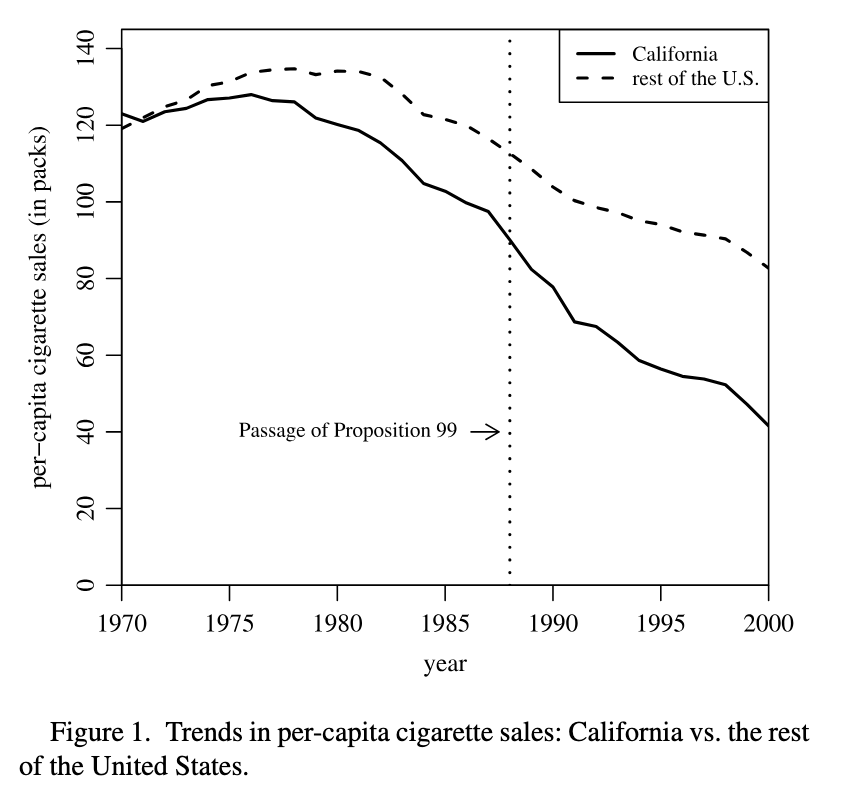
\includegraphics[scale=0.4]{img/fig1.png}
\end{figure}
The rest of the United States may not provide a suitable comparison group for California
\begin{itemize}
    \item Before the ban, cigarette consumption in California differed from the rest of the US
\end{itemize}

% trend similar in the 1970s
% peak in california when the rest of the US was still rising
% When Prop 99 was passed, cigarette consumption was 27% higher in the rest of the country than in California
\end{frame}

%%%%%%%%%%%%%%%%%%%%%%%%%%%%%%%%%%%%%%%%%%%%%%%%%%%%%%%%%%%%%%%%%%%%%%%%%%%%%%%%
\begin{frame}{Building a synthetic California}

Create a donor pool of states from which to build a synthetic California. Include all states that:
\begin{itemize}
    \item Did not adopt large-scale tobacco control programs during the sample period
    \item Did not raise cigarette taxes by 50 cents or more in the post period
\end{itemize}

Construct a synthetic California as a weighted average of potential control states
\begin{itemize}
    \item Weights should be chosen so that the resulting synthetic California best reproduces the values of a set of predictor of cigarette consumption in California before the passage of Prop 99
\end{itemize}

\end{frame}

%%%%%%%%%%%%%%%%%%%%%%%%%%%%%%%%%%%%%%%%%%%%%%%%%%%%%%%%%%%%%%%%%%%%%%%%%%%%%%%%
\begin{frame}{State weights in synthetic California}

\begin{figure}
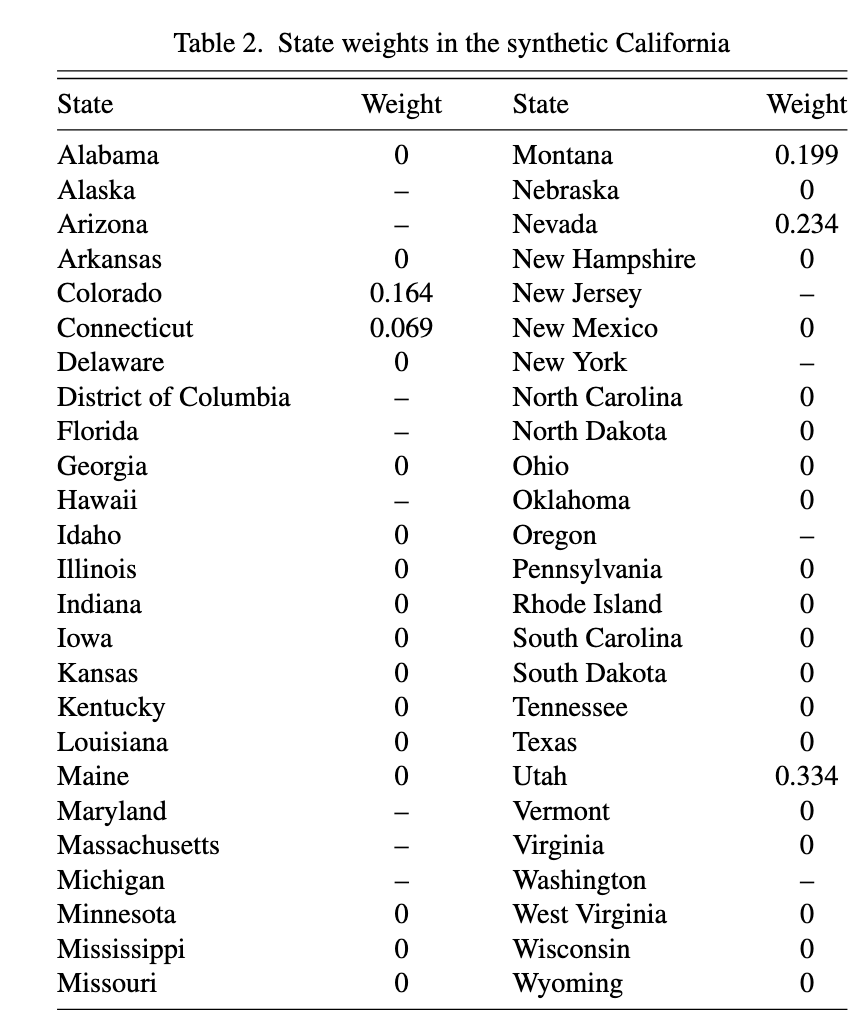
\includegraphics[scale=0.4]{img/table2.png}
\end{figure}


\end{frame}

%%%%%%%%%%%%%%%%%%%%%%%%%%%%%%%%%%%%%%%%%%%%%%%%%%%%%%%%%%%%%%%%%%%%%%%%%%%%%%%%
\begin{frame}{Cigarette sales predictor means}


\begin{figure}
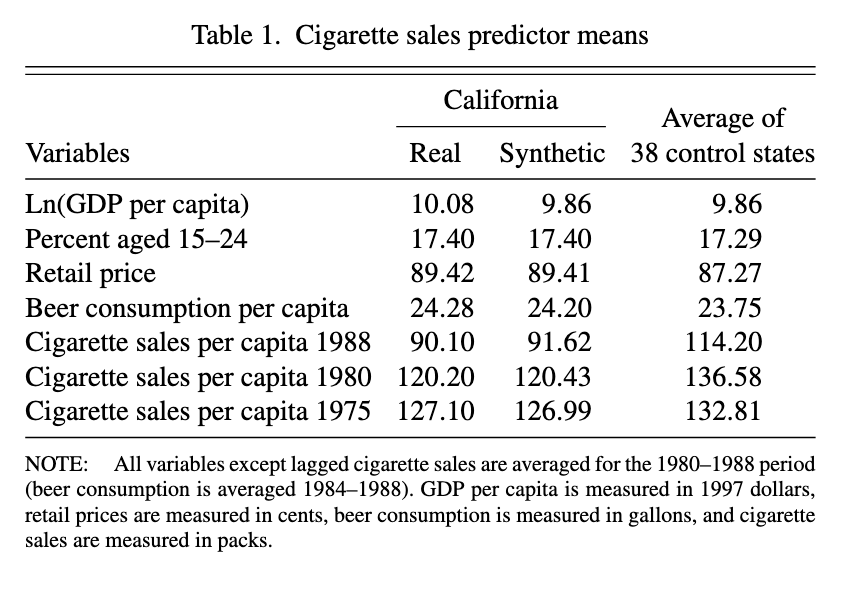
\includegraphics[scale=0.4]{img/table1.png}
\end{figure}


\end{frame}


%%%%%%%%%%%%%%%%%%%%%%%%%%%%%%%%%%%%%%%%%%%%%%%%%%%%%%%%%%%%%%%%%%%%%%%%%%%%%%%%
\begin{frame}{Synthetic California}


\begin{figure}
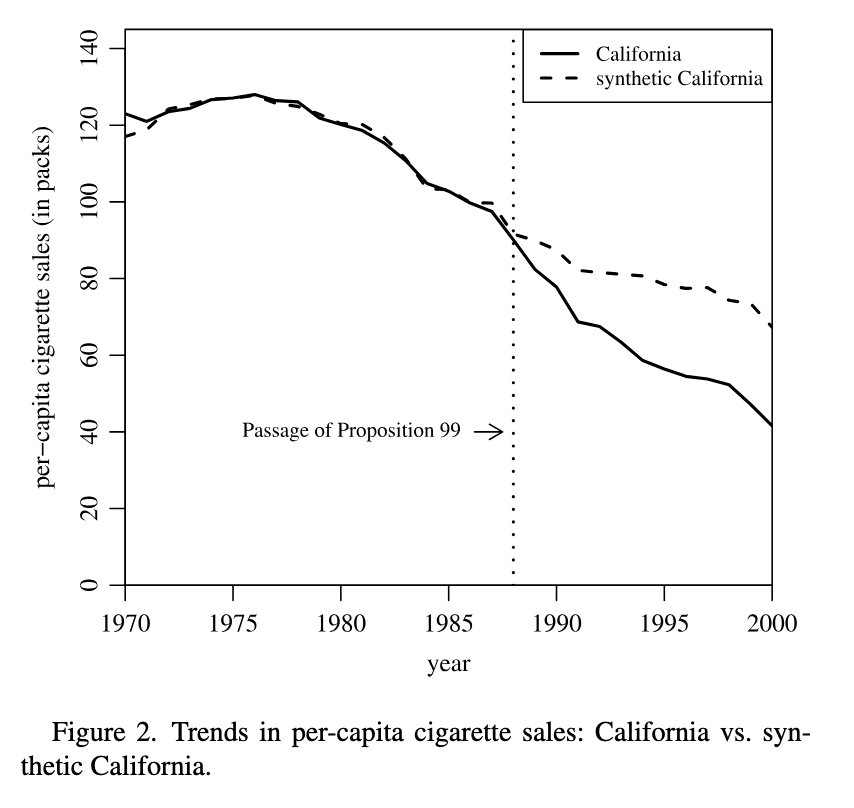
\includegraphics[scale=0.4]{img/fig2.png}
\end{figure}


\end{frame}



%%%%%%%%%%%%%%%%%%%%%%%%%%%%%%%%%%%%%%%%%%%%%%%%%%%%%%%%%%%%%%%%%%%%%%%%%%%%%%%%
\begin{frame}{}

Code available: \url{https://github.com/tara-sullivan/econ726-notebooks/blob/main/notebooks/09-synthetic_control.ipynb}

\end{frame}


%%%%%%%%%%%%%%%%%%%%%%%%%%%%%%%%%%%%%%%%%%%%%%%%%%%%%%%%%%%%%%%%%%%%%%%%%%%%%%%%
\section[Estimation]{Estimating synthetic controls}
\miniframesoff
\begin{frame}
    \tableofcontents[currentsection]
\end{frame}
\miniframeson
%%%%%%%%%%%%%%%%%%%%%%%%%%%%%%%%%%%%%%%%%%%%%%%%%%%%%%%%%%%%%%%%%%%%%%%%%%%%%%%%


%%%%%%%%%%%%%%%%%%%%%%%%%%%%%%%%%%%%%%%%%%%%%%%%%%%%%%%%%%%%%%%%%%%%%%%%%%%%%%%%
\begin{frame}{Defining synthetic $Y_{1t} (0)$}



Synthetic control group defined as weighted average of units in the donor pool, and can be represented by a vector of weights $W = (w_2, \dots, W_{J + 1})$, where
\begin{itemize}
    \item $0 \leq w_i \leq 1$ (No unit receives a negative weight, but units can receive a 0 weight)
    \item $\sum_{i=2}^{J+2} w_i = 1$
\end{itemize}

\vspace{2ex}
Then, for $t=T_0+1, \dots, T$: 
\begin{equation*}
    \hat{Y}_{1t} (0) = \sum_{j=2}^{J+1} w_j Y_{jt}
\end{equation*}

\end{frame}

\begin{frame}{Understanding weights}

Then, for $t=T_0+1, \dots, T$: 
\begin{equation*}
    Y_{1t} (0) = \sum_{j=2}^{J+1} w_j Y_{jt}
\end{equation*}
\begin{figure}
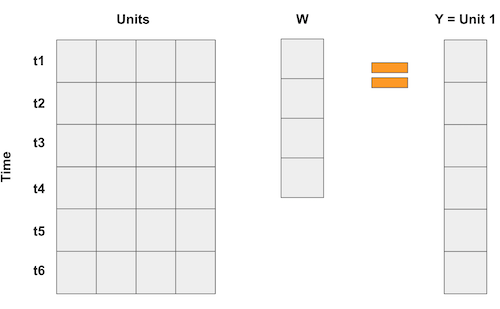
\includegraphics[scale=0.7]{img/weights.png}
\end{figure}

\end{frame}

\begin{frame}{Understanding weights}

For $t=T_0+1, \dots, T$: 
\begin{equation*}
    Y_{1t} (0) = \sum_{j=2}^{J+1} w_j Y_{jt}
\end{equation*}
\begin{figure}
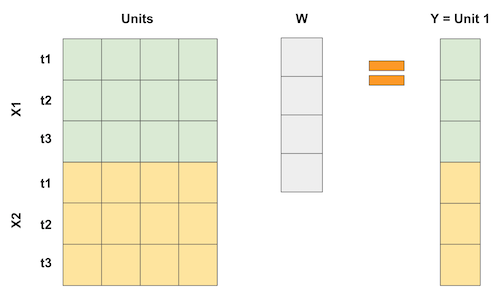
\includegraphics[scale=0.7]{img/weights2.png}
\end{figure}

What if we tried using linear regression for this task?

\end{frame}


%%%%%%%%%%%%%%%%%%%%%%%%%%%%%%%%%%%%%%%%%%%%%%%%%%%%%%%%%%%%%%%%%%%%%%%%%%%%%%%%
\begin{frame}{Interpolation vs extrapolation}

Why $0 \leq w_i \leq 1$ and $\sum_{i=2}^{J+2} w_i = 1$
\begin{figure}
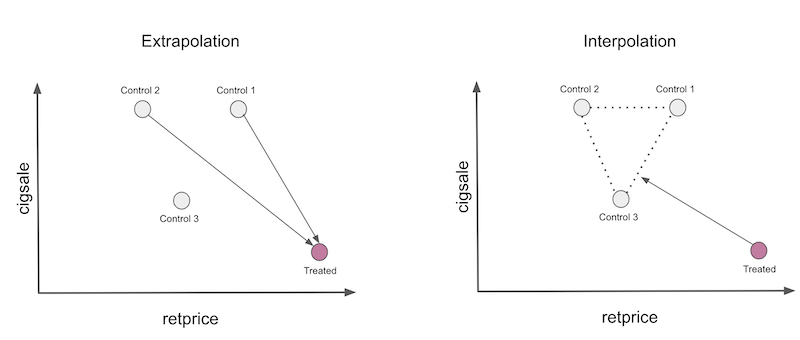
\includegraphics[scale=0.7]{img/extrapolation.png}
\end{figure}


\end{frame}

%%%%%%%%%%%%%%%%%%%%%%%%%%%%%%%%%%%%%%%%%%%%%%%%%%%%%%%%%%%%%%%%%%%%%%%%%%%%%%%%
\begin{frame}{Estimation}

Let:
\begin{itemize}
    \item $X_1$: $k \times 1$ vector of pre-intervention
    characteristics for $i=1$

    \item $X_0$: $k \times J$ matrix with the same characteristics for the control unit
\end{itemize}

Abadie et al. (2010) propose to estimate the synthetic control group such that the distance between pre-treatment characteristics and synthetic control group are minimized:
\begin{align*}
    W^* =& \arg \min_{W} \vert \vert X_1 - X_0 W \vert \vert \\
    \text{ subject to } &\quad 0 \leq w_i \leq 1 \\
    &\quad \sum_{i=2}^{J+1} w_j
\end{align*}
for some norm $\vert\vert \cdot \vert\vert$ (note: a norm is just distance, but in a multivariate space)

\end{frame}

%%%%%%%%%%%%%%%%%%%%%%%%%%%%%%%%%%%%%%%%%%%%%%%%%%%%%%%%%%%%%%%%%%%%%%%%%%%%%%%%
\begin{frame}{}

Weights $W$ can be found by minimizing:
\begin{align*}
    \vert \vert X_1 - X_0 W \vert \vert 
    &= \sqrt{
        (X_1 - X_0 W)^\prime V (X_1 - X_0 W)
    }
\end{align*}
for some symmetric positive definite matrix $k \times k$ matrix $V$. More intuitively, because $V$ is positive definite, its diagonal has values $v1, \dots, v_k$, and this minimization problem looks like:
\begin{equation*}
    \sum_{m=1}^k v_m \left(X_{1m} - \sum_{i=2}^{J+1} w_i X_{im} \right)^2
\end{equation*}
where $v_m$ reflects the relative importance we assign to variable $m$ when we measure the discrepancy between the treated unit and the synthetic control.

\vspace{3ex}
This class is not about numerical optimization, consider examples 

\end{frame}


%%%%%%%%%%%%%%%%%%%%%%%%%%%%%%%%%%%%%%%%%%%%%%%%%%%%%%%%%%%%%%%%%%%%%%%%%%%%%%%%
\section[Inference]{Inference for synthetic controls}
\miniframesoff
\begin{frame}
    \tableofcontents[currentsection]
\end{frame}
\miniframeson
%%%%%%%%%%%%%%%%%%%%%%%%%%%%%%%%%%%%%%%%%%%%%%%%%%%%%%%%%%%%%%%%%%%%%%%%%%%%%%%%



%%%%%%%%%%%%%%%%%%%%%%%%%%%%%%%%%%%%%%%%%%%%%%%%%%%%%%%%%%%%%%%%%%%%%%%%%%%%%%%%
\begin{frame}{Inference}

Could the results from synthetic control be driven by chance?
\begin{itemize}
    \item How often would we obtain results of this magnitude if we had chosen a state at random instead of California?
\end{itemize}

\vspace{3ex}
To answer this, run \textbf{placebo tests}
\begin{itemize}
    \item Apply synthetic control to states that \textbf{did not} implement a large-scale tobacco control program during the sample period

    \item If placebo studies estimate effects similar to the one estimated for the treated unit, then the analysis does not provide significant evidence of a negative effect of Proposition 99 on cigarette sales in California
\end{itemize}

\end{frame}

%%%%%%%%%%%%%%%%%%%%%%%%%%%%%%%%%%%%%%%%%%%%%%%%%%%%%%%%%%%%%%%%%%%%%%%%%%%%%%%%
\begin{frame}{Placebo effects}

Calculate placebo effect for region $i > 1$ at time $t$
\begin{equation*}
    \hat{\alpha}^{*}_{it} = \underbrace{Y_{it} (1)}_{\text{Pretend like $i$ is treated}} - \underbrace{Y_{it} (0)}_{\text{Calculate synthetic control for $i$, as if it were treated}}
\end{equation*}
For each placebo effect for each $i$ (including the actually treated $i=1$), you can calculate the root mean squared error in the pre-intervention period:

\begin{equation*}
    RMSE_{i, pre} = \sqrt{\frac{1}{T_0} \sum_{t=0}^{T_0} \left( 
    % \hat{\alpha}^{*}_{it} 
    Y_{it} - \sum_{j=1}^{J+1} w_j^* Y_{jt}
    \right)^2}
\end{equation*}
\begin{itemize}
    \item For unit $i$, the weights to generate synthetic $i$ are given by $w_j^*$ (for $i=j$, $w_j = 0$)
\end{itemize}
Can also calculate RMSE for each region in the post-intervention period:
\begin{equation*}
    RMSE_{i, post} = \sqrt{\frac{1}{T - T_0} \sum_{t=T_0 + 1}^{T} \left( \hat{\alpha}^{*}_{it} \right)^2}
\end{equation*}



\end{frame}

%%%%%%%%%%%%%%%%%%%%%%%%%%%%%%%%%%%%%%%%%%%%%%%%%%%%%%%%%%%%%%%%%%%%%%%%%%%%%%%%
\begin{frame}{P-value}

Then take the ratio of these errors:
\begin{equation*}
    p_i = \frac{RMSE_{i, post}}{RMSE_{i, pre}}
\end{equation*}
\begin{itemize}
    \item $RMSE_{i, pre}$: How different synthetic $i$ is from real $i$ in the pre-period. We want this small
    \item $RMSE_{i, post}$: How different synthetic $i$ is from real $i$ in the post-treatment period. We expect this to be larger than $RMSE_{i,pre}$
\end{itemize}
Rank ratios from greatest to smallest, and see if the true treated groups p-value is large, relative to the placebo effects

\end{frame}






\end{document}
